%!TEX root = ../thesis.tex
%******************************************************************************
\chapter{An Adaptive Middleware for Near-Time Processing of Bulk Data}\label{ch:adaptive_middleware}
%******************************************************************************

\section{Introduction}\label{sec:introduction}
Enterprise Systems like customer-billing systems or financial transaction systems are required to process large volumes of data in a fixed period of time. For example, a billing system for a large telecommunication provider has to process more than 1 million bills per day.
Those systems are increasingly required to also provide near-time processing of data to support new service offerings.

Traditionally, enterprise systems for bulk data processing are implemented as batch processing systems \citep{Fleck:1999aa}. Batch processing delivers high throughput but cannot provide near-time processing of data, that is the end-to-end latency of such a system is high. End-to-end latency refers to the period of time that it takes for a business process, implemented by multiple subsystems, to process a single business event.  For example, consider the following billing system of telecommunications provider:
\begin{itemize}
	\item Customers are billed once per month
	\item Customers are partitioned in 30 billing groups
	\item The billing system processes 1 billing group per day, running 24h under full load.
\end{itemize}
In this case, the mean time for a call event to be billed by the billing system is 1/2 month. That is, the mean end-to-end latency of this system is 1/2 month.

A lower end-to-end latency can be achieved by using single-event processing, for example by utilizing a message-oriented middleware for the integration of the services that form the enterprise system. While this approach is able to deliver near-time processing, it is hardly capable for bulk data processing due to the additional communication overhead for each processed message. Therefore, message-based processing is usually not considered for building a system for bulk data processing requiring high throughput.

The processing type is usually a fixed property of an enterprise system that is decided when the architecture of the system is designed, prior to implementing the system. This choice depends on the non-functional requirements of the system. These requirements are not fixed and can change during the lifespan of a system, either anticipated or not anticipated.

Additionally, enterprise systems often need to handle load peaks that occur infrequently. For example, think of a billing system with moderate load over most of the time, but there are certain events with very high load such as New Year's Eve. Most of the time, a low end-to-end latency of the system is preferable when the system faces moderate load. During the peak load, it is more important that the system can handle the load at all. A low end-to-end latency is not as important as an optimized maximum throughput in this situation.

In this paper, we propose a solution to this problem:

\begin{itemize}
	\item We introduce the concept of a middleware that is able to adapt its processing type fluently between batch processing and single-event processing. By adjusting the data granularity at runtime, the system is able to minimize the end-to-end latency for different load scenarios. (Section \ref{sec:adaptive_middleware})
\end{itemize}

The remainder of this paper is organized as follows. Section \ref{sec:background} defines the considered type of system and the terms throughput and latency. The proposed middleware and the results of preliminary performance tests are presented in Section \ref{sec:adaptive_middleware}. Section \ref{sec:related_work} gives an overview of other work related to this reasearch. Finally, Section \ref{sec:conclusion} concludes the paper and gives and outlook to the next steps of this research.

\section{Background}\label{sec:background}
We consider a distributed system for bulk data processing consisting of several subsystems running on different nodes that together form a processing chain, that is, the output of subsystem S1 is the input of the next subsystem S2 and so on (see Figure \ref{fig:system_single}).
\begin{figure}[h!]
	\centering
	\mbox{\subfloat[Single processing line]{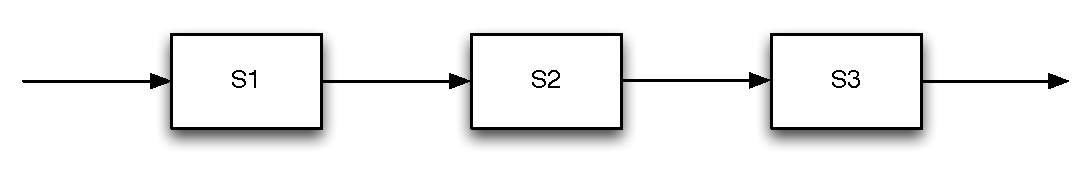
\includegraphics[width=\columnwidth]{considered_system_single}\label{fig:system_single}}}
	\mbox{\subfloat[Parallel processing lines]{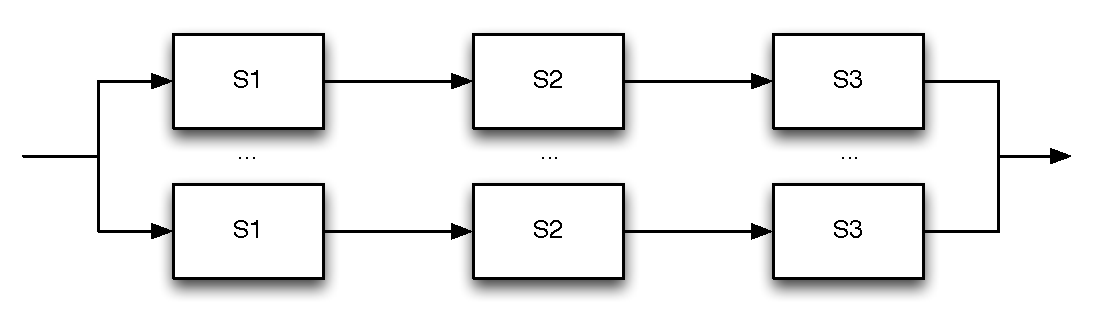
\includegraphics[width=\columnwidth]{considered_system_parallel}\label{fig:sytem_parallel}}}
	\caption{A system consisting of several subsystems forming a processing chain}
\end{figure}

To facilitate parallel processing, the system can consist of several lines of subsystems with data beeing distributed among each line. For simplification, we consider a system with a single processing line in the remainder of this paper.

We discuss two processing types for this kind of system, batch processing and message-based processing.
\subsection{Batch processing}
The traditional operation paradigm of a system for bulk data processing is batch processing (see Figure \ref{fig:batch_processing}). A batch processing system is an application that processes bulk data without user interaction. Input and output data is usually organized in records using a file- or database-based interface. In the case of a file-based interface, the application reads a record from the input file, processes it and writes the record to the output file.
\begin{figure}[h!]
	\centering
	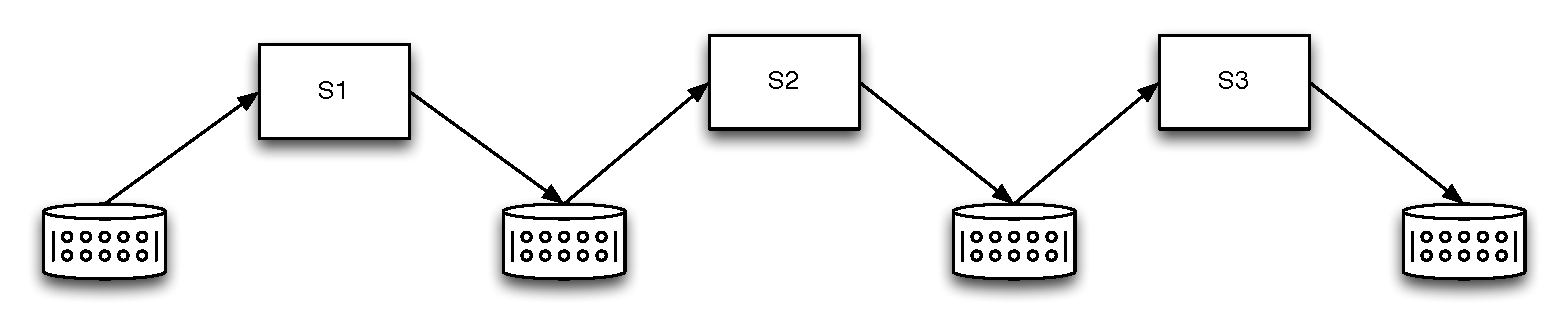
\includegraphics[width=\columnwidth]{batch_processing}
	\caption{Batch processing}
	\label{fig:batch_processing}
\end{figure}

\subsection{Message-base processing}
Messaging facilitates the integration of heterogeneous applications using asynchronous communication. Applications are communicating with each other by sending messages (see Figure \ref{fig:message_based_processing}). A messaging server or message-oriented middleware handles the asynchronous exchange of messages including an appropriate transaction control \citep{conrad2006enterprise}.

\begin{figure}[h!]
	\centering
	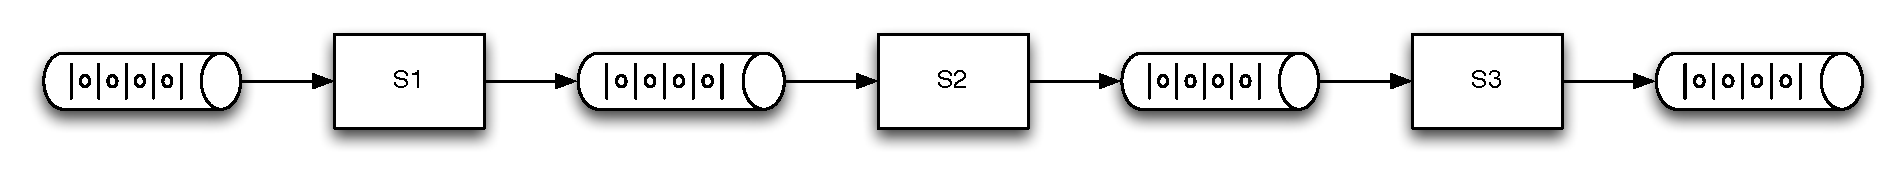
\includegraphics[width=\columnwidth]{message_processing}
	\caption{Message-based processing}
	\label{fig:message_based_processing}
\end{figure}

Message-based systems are able to provide near-time processing of data due to their lower latency compared with batch processing systems. The advantage of a lower latency comes with a performance cost in regard to a lower maximum throughput because of the additional overhead for each processed message. Every message needs, amongst others, to be serialized and deserialized, mapped between different protocols and routed to the appropriate receiving system.

\subsection{End-to-end Latency vs. Maximum Throughput}\label{sec:latency_throughput}
Throughput and latency are performance metrics of a system. We are using the following definitions of maximum throughput and latency in this paper:
\begin{itemize}
	\item \textbf{Maximum Throughput}\\
	The number of events the system is able to process in a fixed timeframe.
 	\item \textbf{End-To-End Latency}\\
	The period of time between the occurrence of an event and its processing. End-to-end latency refers to the total latency of a complete business process implemented by multiple subsystems. The remainder of this paper focusses on end-to-end latency using the general term latency as an abbreviation.
\end{itemize}

Latency and maximum throughput are opposed to each other given a fixed amount of processing resources. High maximum throughput, as provided by batch processing, leads to high latency, which impedes near-time processing. On the other hand, low latency, as provided by a message-based system, cannot provide the maximum throughput needed for bulk data processing because of the additional overhead for each processed event.

\section{An adaptive middleware for near-time processing of bulk data}\label{sec:adaptive_middleware}
This section introduces the concept of an adaptive middleware which is able to adapt its processing type fluently between batch processing and single-event processing. It continuously monitors the load of the system and controls the message aggregation size. Depending on the current aggregation size, the middleware automatically chooses the appropriate service implementation and transport mechanism to further optimize the processing.
\subsection{Middleware Components}
Figure \ref{fig:middleware_components} shows the components of the middleware, that are based on the Enterprise Integration Patterns described by \cite{Hohpe:2003fk}.

\begin{figure*}[!t]
	\centering
	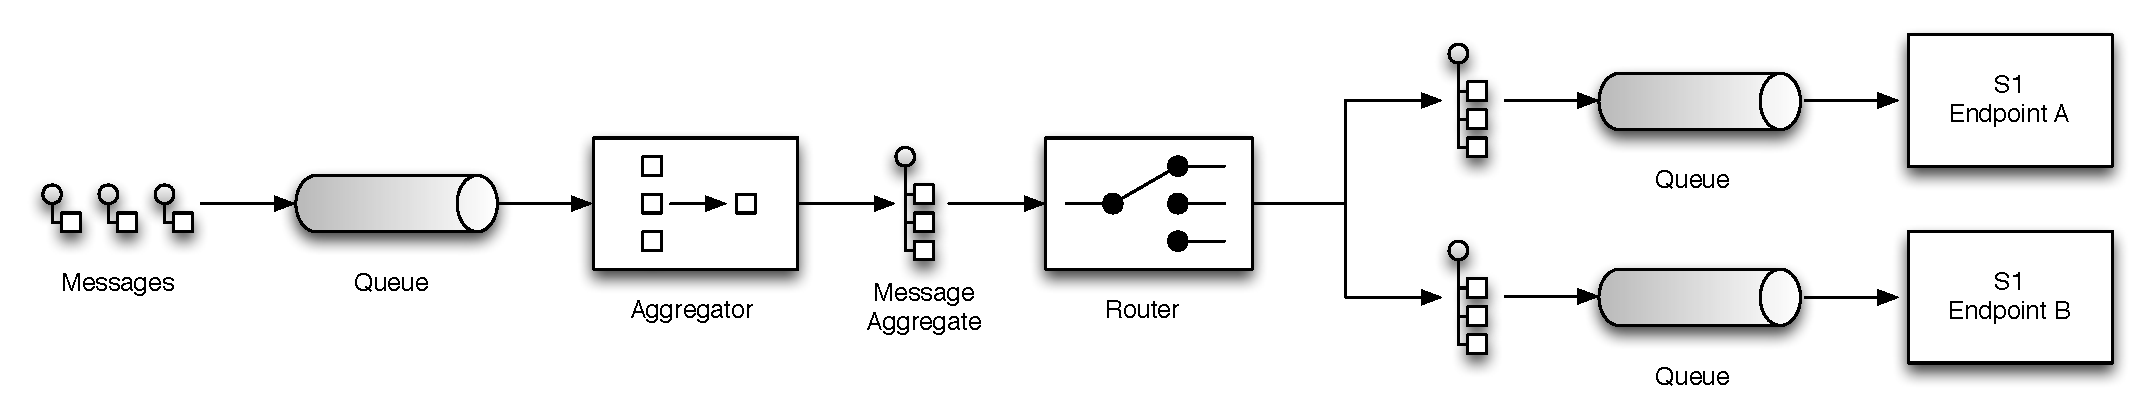
\includegraphics[width=\textwidth]{middleware_components}
	\caption{Components of the Adaptive Middleware. We are using the notation defined by \cite{Hohpe:2003fk}}
	\label{fig:middleware_components}
\end{figure*}

\subsubsection{Aggregator}
The Aggregator is a stateful filter which stores correlated messages until a set of messages is complete and sends this set to the next processing stage in the messaging route. 

There are different options to aggregate messages, which can be implemented by the Aggregator:

\begin{itemize}
	\item \textbf{No correlation}: Messages are aggregated in the order in which they are read from the input message queue. In this case, an optimized processing is not simply possible.
	\item \textbf{Technical correlation:} Messages are aggregated by their technical properties, for example by message size or message format.
	\item \textbf{Business correlation}: Messages are aggregated by business rules, for example by customer segments or product segments.
\end{itemize}

\subsubsection{Feedback Loop}

To control the level of message aggregation at runtime, the middleware uses a closed feedback loop with the following properties (see Figure \ref{fig:feedback_loop}):

\begin{itemize}
	\item \textbf{Input (u):} Current aggregation size
	\item \textbf{Output (y):} Change of queue size measured between sampling intervals
	\item \textbf{Set point (r):} The change of queue size should be zero.
\end{itemize}

Ultimately, we want to control the average end-to-end latency depending on the current load of the system. The change of queue size seems to be an appropriate quantity because it can be directly measured without a lag at each sampling interval, unlike the average end-to-end latency.

\begin{figure}[htbp]
	\centering
	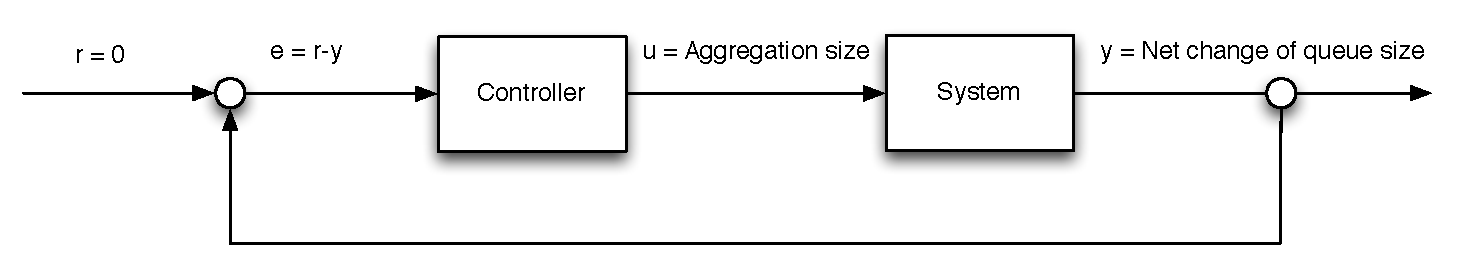
\includegraphics[width=\columnwidth]{feedback_loop}
	\caption{Feedback loop to control the aggregation size}
	\label{fig:feedback_loop}
\end{figure}
The concrete architecture and tuning of the feedback loop and the controller is subject to our ongoing research.
\subsubsection{Router}
Depending on the size of the aggregated message, the Router routes the message to the appropriate service endpoint, which is either optimized for batch or single event processing.

When processing data in batches, especially when a batch contains correlated data, there are multiple ways to speed up the processing:
\begin{itemize}
	\item To reduce I/O, data can be pre-loaded at the beginning of the batch job and held in memory.
	\item Storing calculated results for re-use in memory
	\item Use bulk database operations for reading and writing data
\end{itemize}

With high levels of message aggregation, it is not preferred to send the aggregated message payload itself over the message bus using Java Message Service (JMS) or SOAP. Instead, the message only contains a pointer to the data payload, which is transferred using File Transfer Protocol (FTP) or a shared database.

\subsection{Service Design}

\subsection{Controller Design}

\subsubsection{Control Problem}

\subsubsection{Input/Output Variables}

\subsubsection{Control Strategy}

\subsection{Error Handling}

\section{Prototype Implementation}
To evaluate the proposed concepts of the adaptive middleware, we have implemented a prototype of a billing system using Apache Camel \citep{apachecamel} as the messaging middleware.

Figure \ref{fig:message_prototype} shows the architecture of the prototype system.

\begin{figure}[h!]
	\centering
	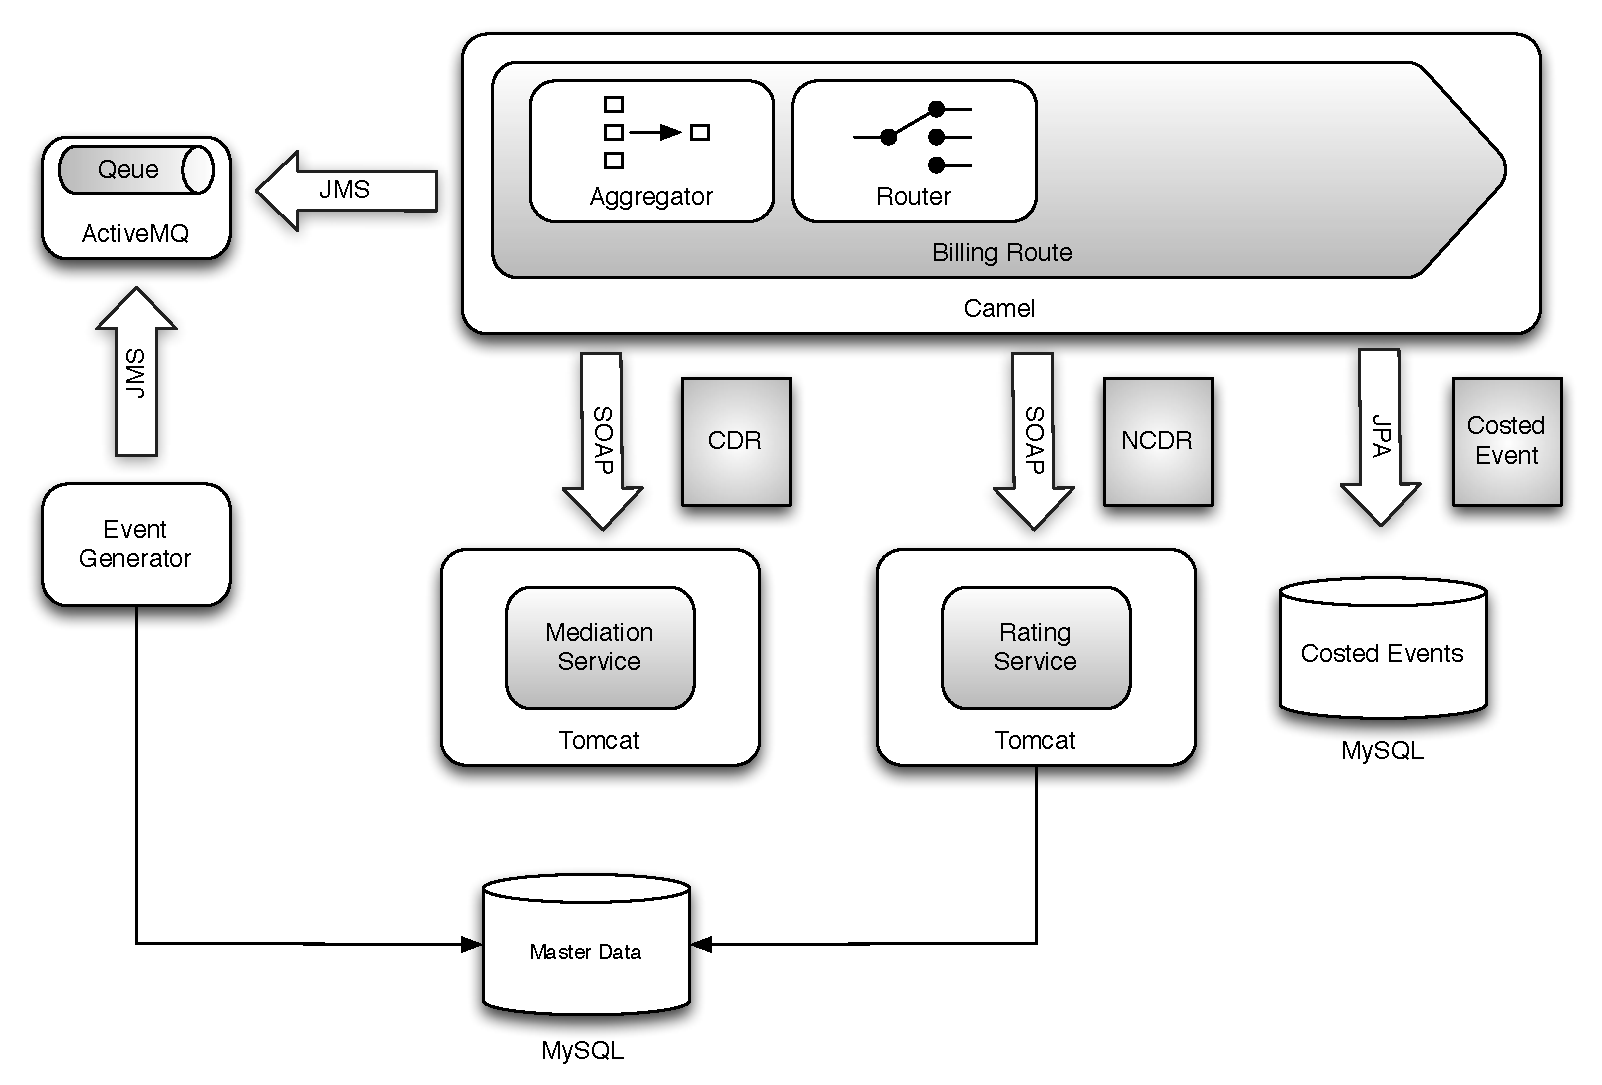
\includegraphics[width=\columnwidth]{prototype}
	\caption{Architecture of the prototype system}
	\label{fig:message_prototype}
\end{figure}

Using this prototype, we have done some preliminary performance tests to examine the impact of message aggregation on latency and throughput. For each test, the input message queue has been pre-filled with 100.000 events. We have measured the total processing time and the processing time of each message with different static message aggregation sizes.

Figure \ref{fig:throughput_aggregation} shows the impact of different aggregation sizes on the throughput of the messaging prototype.
\begin{figure}[htbp]
	\centering
	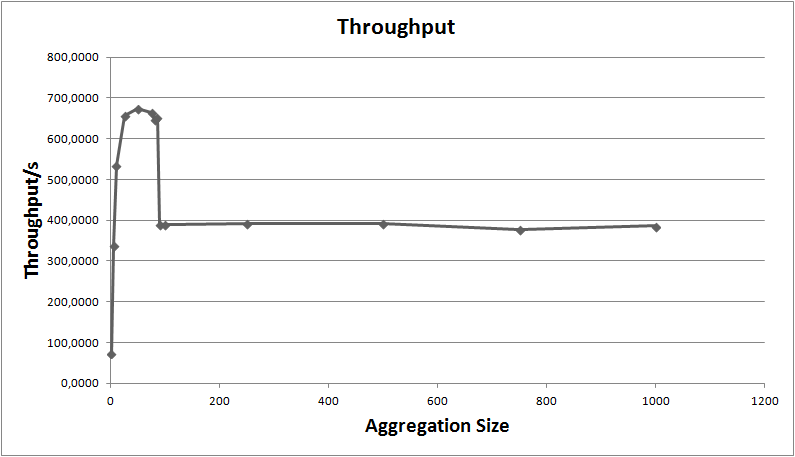
\includegraphics[width=\columnwidth]{throughput_aggregation}
	\caption{Impact of different aggregation sizes on throughput}
	\label{fig:throughput_aggregation}
\end{figure}
The throughput increases constantly for $1<aggregation\_size<=50$ with a maximum of 673 events per second with $aggregation\_size=50$. Higher aggregation sizes than 50 do not further increase the throughput, it stays around 390 events per second.

The increased throughput achieved by increasing the aggregation size comes with the cost of a higher latency. Figure \ref{fig:latency_aggregation} shows the impact of different aggregation sizes on the 95th percentile latency of the messaging prototype. 
\begin{figure}[htbp]
	\centering
	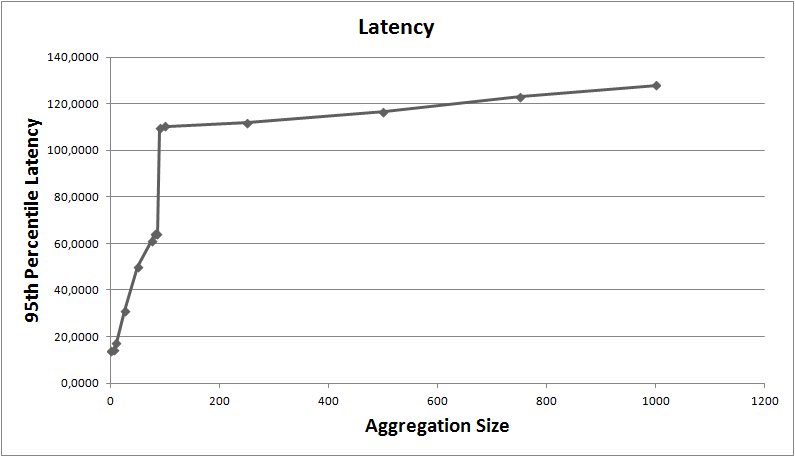
\includegraphics[width=\columnwidth]{latency_aggregation}
	\caption{Impact of different aggregation sizes on latency}
	\label{fig:latency_aggregation}
\end{figure}

An aggregation size of 50, resulting in the maximum throughput of 673 events per seconds, shows a 95th percentile latency of about 68 seconds.

The results indicate that there is an optimal range for the aggregation size to control the throughput and latency of the system. Setting the aggregation size higher than a certain threshold leads to a throughput drop and latency gain. In case of our prototype, this threshold is between an aggregation size of 85 and 90. This threshold needs to be considered by the control strategy. We are currently investigating the detailed causes of this finding.

\section{Evaluation}

\section{Related Work}\label{sec:related_work}
Research on messaging middleware currently focusses on Enterprise Services Bus (ESB) infrastructure. An ESB is an integration plattform that combines messaging, web services, data transformation and intelligent routing to connect multiple heterogeneous services \citep{Chappell:2004jo}. It is a common middleware to implement the integration layer of an Service Oriented Architecture (SOA) and is available in numerous commercial and open-source packages.

Several research has been done to extend the static service composition and routing features of standard ESB implementations with dynamic capabilities decided at run-time, such as dynamic service composition \citep{Chang:2007aa}, routing \citep{Bai:2007aa} \citep{Wu:2008aa} \citep{Ziyaeva:2008aa} and load balancing \citep{Jongtaveesataporn:2010aa}.

Work to manage and improve the Quality of Service (QoS) of ESB and service-based systems in general is mainly focussed on dynamic service composition and service selection based on monitored QoS metrics such as throughput, availability and response time \citep{Calinescu:2011aa}. \cite{Gonzalez:2011} propose an adaptive ESB infrastructure to adress QoS issues in service-based systems which provides adaption strategies for response time degradation and service saturation, such as invoking an equivalent service, using previously stored information, distributing requests to equivalent services, load balancing and deferring service requests.

The adaption strategy of our middleware is to change the message aggregation size based on the current load of the system. Aggregating or batching of messages is a common approach to increase the throughput of a messaging system, for example to increase the throughput of total ordering protocols \citep{Friedman:1997aa} \citep{Friedman:2006aa} \citep{Romano:2012aa} \citep{Didona:2012aa}.

A different solution to handle infrequent load spikes is to automatically instantiate additional server instances, as provided by current Platform as a Service (PaaS) offerings such as Amazon EC2 \citep{ec2_autoscaling} or Google App Engine \citep{google_cloud_autoscaling}. While scaling is a common approach to improve the performance of a system, it also leads to additional operational and possible license costs. Of course, our solution can be combined with these auto-scaling approaches.

\section{Conclusion and Future Work}\label{sec:conclusion}
In this paper, we have presented a middleware that is able to adapt itself to changing load scenarios by fluently shifting the processing type between single event and batch processing. The middleware uses a closed feedback loop to control the end-to-end latency of the system by adjusting the level of message aggregation depending on the current load of the system. Determined by the aggregation size of a messsage, the middleware routes a message to appropriate service endpoints, which are optimized for either single-event or batch processing.

To evaluate the proposed middleware concepts, we have implemented a prototype system and performed preliminary performance tests. The tests show that throughput and latency of a messaging system depend on the level of data granularity and that the throughput can be increased by increasing the granularity of the processed messages.

Next steps of our research are the implementation of the proposed middleware including the evaluation and tuning of different controller architectures, performance evaluation of the proposed middleware using the prototype and developing a conceptional framework containing guidelines and rules for the practitioner how to implement an enterprise system based on the adaptive middleware for near-time processing
